\normalsize\subsection{Definizioni di acido e base}
Le definizioni di acidi e basi sono variate negli anni.

Inizialmente abbiamo classificato come acido o base un dato composto in funzione dell'elettronegatività dell'atomo X nella seguente reazione

$$\ce{XOH(aq) + H_2O -> XO^-(aq) + H_3O^+(aq)}, \quad \text{X elettronegativo}$$

$$\ce{XOH(aq) + H_2O -> X^+(aq) + OH^-(aq)}, \quad \text{X elettropositivo}$$

Immaginiamo quindi di avere un generico composto formato da un atomo X con almeno un gruppo OH.

Alcuni composti liberano il loro idrogeno sotto forma di H$^+$, cioè in essi si rompe il legame ossigeno-idrogeno, altri invece liberano il gruppo O-H sotto forma di OH$^-$, cioè si rompe il legame X-OH. Quindi in funzione dell'elettronegatività dell'atomo X si può vedere quale sia il legame più facile da rompere in acqua:

\begin{itemize}
    \item Se il composto libera ioni H$^+$ diciamo che è \textbf{acido};
    \item Se il composto libera ioni OH$^-$ diciamo che è una \textbf{base}.
\end{itemize}

\subsubsection{Definizione di Arrhenius (1887)}
La definizione finora adoperata è stata enunciata da Arrhenius, il quale etichettò come acido una qualunque specie chimica che in acqua libera ioni H$^+$ e come base una qualunque specie chimica che in acqua libera ioni OH$^-$.

\vspace{0.2cm}Esempi di acidi:

\vspace{0.2cm}\ce{HCl(aq) + H_2O -> H^+(aq) + Cl^-(aq)}

\vspace{0.2cm}\ce{H_2SO_4(aq) + H_2O -> H^+(aq) + H_2SO_4^-}

\vspace{0.2cm}\ce{H_2SO_4^- + H_2O -> H^+(aq) + SO_4^{2-}}

\vspace{0.2cm}Esempi di basi:

\vspace{0.2cm}\ce{NaOH(aq) -> Na^+(aq) + OH^-(aq)}

\vspace{0.2cm}\ce{Ba(OH)_2(aq) -> Ba(OH)^+(aq) + OH^-(aq)}

\vspace{0.2cm}\ce{Ba(OH)^+ -> Ba^{2+}(aq) + OH^-(aq)}

\vspace{0.2cm}Questa definzione però pone due limiti:

\begin{enumerate}
    \item Si considera solo l'acqua come solvente, per cui se questi composti fossero in solventi diversi non avremmo modo di etichettarli.
    \item Ci sono delle incongruenze. Ad esempio l'ammoniaca NH$_3$ che è una base non ha ioni OH$^-$ da liberare, pertanto secondo questa definizione non potrebbe essere una base.
\end{enumerate}
\subsubsection{Definizione di Brönsted-Lowry (1923)}
Si giunse quindi alla teoria acido-base di Brönsted-Lowry. Con essa si etichetta acido ogni specie chimica che è in grado di donare protoni.

\vspace{0.2cm}esempi di acidi di Brönsted-Lowry

\vspace{0.2cm}\ce{CH_3COOH(aq) + H_2O <--> CH_3COO^-(aq) + H_3O^+}

acido acetico \hspace{2.55cm} ione acetato 

\vspace{0.2cm}\ce{NH_4^+(aq) + H_2O <--> NH_3(aq) + H_3O^+(aq}

ione ammonio \hspace{1.35cm} ammoniaca

\vspace{0.2cm}\ce{H_2PO_4^-(aq) + H_2O <--> H_2PO_4^{2-}(aq) + H_3O^+(aq)}

ione fosfato \hspace{2.25cm} ione fosfato

acido \hspace{3.4cm} bi-acido

\vspace{0.2cm}Lo ione H$^+$ è scritto come H$_3$O$^+$, ossia lo ione H$^+$ si addiziona ad una molecola di acqua per dar luogo a H$_3$O$^+$. Scrivere così ci indica che il ruolo del solvente diventa determinante. Dunque in acqua lo ione H$^+$ non esiste come tale, ma si somma all'acqua.

Va poi da ricordare che se scrivessimo la molecola dell'acqua secondo la teoria di Lewis, sull'ossigeno resterebbero due doppietti non coinvolti nel legame chimico. Uno di questi due è molto interno, cioè ad energia molto negativa, pertanto non è disponibile per formare legame chimico; l'altro invece è esterno in energia, quindi è disponibile a essere coinvolto nel formare alrri legami. Questo doppietto permette infatti la formazione di un \textbf{legame dativo}, ossia un legame dovuto non ad una messa in comune di elettroni da parte dei due partners, ma al fatto che uno dei due fornisce entrambi gli elettroni necessari. In questo caso i due elettroni necessari sono costituiti dal doppietto dell'ossigeno.

Inoltre in tutti e tre i casi stiamo parlando di equilibri (c'è la doppia freccia), quindi non di reazioni spostate verso destra.

\vspace{0.2cm}Secondo questa teoria poi, si definisce base ogni specie chimica che è in gradi di accettare protoni.

\vspace{0.2cm}Esempi di basi di Brönsted-Lowry

\vspace{0.2cm}\ce{NH_3(aq) + H_2O <--> NH_4^+(aq) + OH^-(aq)}

\vspace{0.2cm}Se l'ammoniaca accetta un protone dall'acqua diventa ione ammonio e l'aqua che ha perso un protone diventa ione OH$^-$. Stavolta allora il protone sarà ceduto dall'acqua. Ne segue che, siccome l'NH$_3$ ha accettato un protone, è una base, mentre l'acqua si è comportata da acido perché sta cedendo un protone. Al contrario, nelle reazioni precedenti l'acqua stava acquistando il protone delle speci chimiche.

L'acqua allora divents determinante: non è più solo il solvente, ma si può comportare da base o da acido a seconda della reazione. Tale è fatto è ciò che sfuggiva ad Arrhenius.

\vspace{0.2cm}\ce{CO_3^{2-}(aq) + H_2O <--> HCO_3^- + OH^-(aq)}

\vspace{0.2cm}Lo ione carbonato CO$_3^{2-}$ è una base perché accetta un protone strappandolo all'acqua. Accetta quindi uno ione H$^+$ diventando ione bicarbonato HCO$_3^-$ e lasciando OH$^-$. Secondo la teoria di Arrhenius il carbonato non poteva essere etichettato base, perché non ha ioni OH$^-$ da mandare in soluzione, analogamente all'ammoniaca.

Spesso, quando dopo mangiato abbiamo una sensazione di acidità, usiamo il bicarbonato perché esso consuma l'eccesso di acido che abbiamo nello stomaco formando H$_2$CO$_3$, cioè quindi consumando gli ioni H$^+$. Dunque anche la specie HCO$_3^-$ è una base.

\subsubsection{Definizione di Lewis (1923)}
In larga misura useremo la definizione di Brönsted-Lowry per acidi e basi. Tuttavia ne esiste una ancora più ampia, che è la definizione di Lewis. Con essa si definisce acido una specie in grado di accettare coppie di elettroni, che più o meno è la stessa cosa: se si libera uno one H$^+$ restano elettroni sulla specie che libera questi protoni, e quindi è come se stesse accettando una coppia di elettroni. Si definisce invece base una specie che può cedere coppie di elettroni.

\vspace{0.2cm}Esempi:

\vspace{0.2cm}\chemfig{\charge{[circle]0=\:}{H_3N}} \ce{+ H^+ <--> NH_4^+}

\vspace{0.2cm}L'ammoniaca ha un doppietto sull'azoto chd usa per legare lo ione H$^+$ che sta strappando all'acqua per formare la specie NH$_4^+$.

Chiaramente per legare lo ione H$^+$ cede questi due elettroni, mettendoli in comune, quindi l'ammoniaca continua ad essere base anche secondo la definizione di Lewis

\vspace{0.2cm}\chemfig{\charge{[circle]0=\:}{H_3N}} \ce{+ BF_3 <-->}\chemfig{\charge{[circle]0=\:}{H_3N}} \ce{\bond{->}BF_3}

\vspace{0.2cm}In questa reazione nei prodotti c'è una freccia che sta a indicare la formazione di un legame dativo: entrambi gli elettroni vengono messi in comune dall'azoto.

Prodotti di questo tipo si chiamano \textbf{addotti}. In questo caso abbiamo un addotto tra NH$_3$ e BF$_3$.

In questa reazione abbiamo una specie in grado di cedere elettroni, che è la base, e la specie BF$_3$ che è in grado di acquistare cioè accettare coppie di elettroni. Secondo la teoria dell'ibridizzazione, il BF$_3$ ha ibridi $\rm sp^2$ utilizzati tutti e tre dal boro per formare i tre legami col fluoro. Restava però un terzo orbitale p non ibridizzato perpendicolare al piano della molecola a disposizione.

Il boro ha 3 elettroni, 2 nell'orbitale 2s e solo uno negli orbitali p. Parlavamo quindi di stato di promozione così da avere un elettrone nell'orbitale s e 2 elettroni in due diversi orbitali p. Avevamo quindi 3 orbitali occupati singolarmente e uno no. Con la reotira dell'ibridizzazione immaginavamo poi che i tre orbitali occupati si mescolassero tra loro per dare luogo a tre ibridi $\rm sp^2$, ognuno dei quali con 1 elettrone. Formavamo quindi i 3 legami del BF$_3$, ma sul boro resta totalmente vuoto un orbitale p non ibridizzato perpendicolare al piano della molecola. Esso sarà quello in grado di accettare la coppia di elettroni, cioè il doppietto dell'azoto, interagirà con questo orbitale, formando un nuovo legame chimico. Ciò che allora succede è che l'ammoniaca sta cedendo degli elettroni e il BF$_3$ li sta acquistando, pertanto secondo questa teoria quest'ultimo è un acido, cosa che nei fatti è.

\vspace{0.2cm}Etichettiamo quindi con \textit{reazione acido-base} la formazione di un legame chimico tra NH$_3$ e BF$_3$, tenendo presente la teoria di Lewis.

\vspace{0.2cm}Abbiamo visto che con la teoria di  Br\"{o}nsted-Lowry l'acqua partecipa attivamente alla reazione, comportandosi a volte come acido e a volte come base in funzione del partner. Secondo la teoria di Lewis l'acqua è etichettata come \textit{base di Lewis} e il protone (cioè lo ione H$^+$) come \textit{acido di Lewis}. La loro unione ci dà un addotto.

Quindi tutte le volte in cui la coppia di elettroni di legame viene messa in comune solo da uno dei due partner si forma un legame dativo e il composto ottenuto viene chiamato addotto.

Anche l'ammoniaca è una base di Lewis, e se ad essa sommiamo un acido di Lewis dà luogo allo ione ammonio:

\begin{figure}[htp]
    \centering
    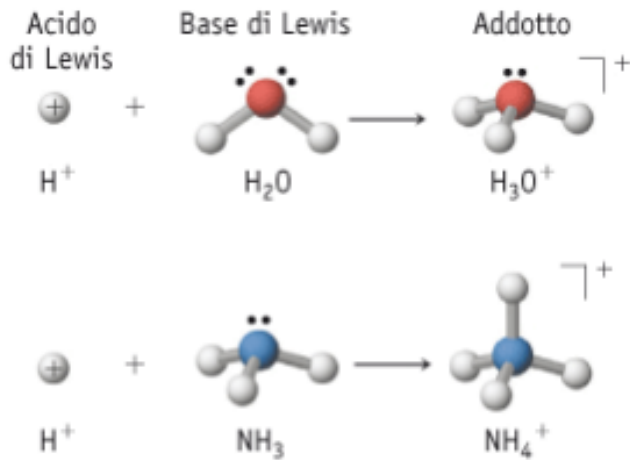
\includegraphics[width=8cm]{immagini/acidi_e_basi_di_lewis.png}
\end{figure}

\subsection{Ioni complessi in soluzione acquosa}
Entriamo ora più nel dettaglio per quella che la teoria etichetta \textit{coppia coniugata acido-base}. Va da precisare infatti che, similmente a quanto dicevamo per le redox dove non può esistere un ossidante se non c'è constestualmente il riducente, nelle reazioni acido base se una specie perde elettroni è indispensabile che questi vengano acquistati da un'altra specie. Lo stesso vale per gli acidi e le basi: affinché una specie assuma il comportamente di acido deve essere in presenza di una base.

Secondo Br\"{o}nsted-Lowry se c'è una specie che cede un protone ci vuole una specie che acquisti questo protone. Quindi non c'è un acido o una base, ma abbiamo sempre coppie coniugate acido-base.

\vspace{0.2cm}Se mettiamo sei sali neutri in acqua, questi si dissociano e il catione viene coordinato, cioè circondato in maniera ordinata, da molecole di acqua, formando un complesso di forma diversa in base al numero di molecole d'acqua necessarie. In generale si parla di \textbf{poliedro di coordinazione}.

Inoltre questi complessi danno luogo a soluzioni colorate, sebbene i sali anidri (cioè senza acqua) non presentano tali colorazioni. Il colore è dovuto allora al complesso che si forma. La reazione del catione metallico e un certo numero di molecole di acqua è una reazione acido-base: l'acqua è il doppietto ed è la base di Lewis, lo ione metallico ha orbitali vuoti e quindi può accettare coppie di elettroni, pertanto è l'acido di Lewis.

\vspace{0.2cm}Esempi:

$$\ce{Be^{2+}(aq) + 4H_2O(l) <--> [Be(H_2O)_4]^{2+}(aq)}$$

Questo ione viene coordinato da 4 molecole d'acqua, formando un complesso tetraedrico, ossia gli ossigeni dell'H$_2$O sono disposti ai vertici di un tetraedro Quindi in acqua non c'è un mescolamento casuale, si formano delle geometrie ben precise nei complessi. Le molecole di acqua costituiscono l'\textit{intorno di coordinazione}.

Anche in questo esempio lo ione berillio è un acido di Lewis e l'acqua è la base di Lewis.

\subsection{Lo ione idronio H$_3$O$^+$}
Abbiamo detto che etichettiamo acidi i composti che cedono un protone. Possiamo allora immaginare che l'idrogeno diventi H$^+$ più un elettrone e$^-$.

Il protone H$^+$ ha dimensioni di 0.0015 pm, mentre gli atomi hanno dimensioni tra i 50 e i 200 pm, ciononostante la sua carica è comunque +1 come quella di uno ione. Ne segue che il rapporto tra carica e raggio per l'H$^+$ è molto più grande di quello degli ioni. A causa di ciò, il protone non può esistere da solo in un liquido o in un solido: si associa a qualunque cosa pur di diminuire il rapporto carica raggio.

In acqua si associa ad una molecola d'acqua per formare lo ione idronio $\rm H_3O^+$. Così facendo la carica resta +1 ma le dimensioni della molecola crescono.

$$\ce{H^+(g) + H_2O(g) <--> H_3O^+(gas)}$$

Quando questa reazione avviene, vista l'elevata tendenza del protone ad associarsi con altre specie chimiche per ridurre il rapporto carica raggio, si liberano 720 kJ/mol.

Va da ricordare che quando l'idrogeno perde un protone ha un potenziale di ionizzazione di 1311 kJ/mol (\ce{H <--> H^+ + e^-}).

\vspace{0.2cm}Consideriamo adesso la stessa reazione in acqua liquida:

$$\ce{H^+(g) + H_2O(l) <--> H_3O^+(aq)}$$

In questo caso lo ione H$^+$ gassoso viene catturato da dell'acqua liquida per formare lo ione $\rm H_3O^+$ in acqua, quindi il protone gassoso si idrata perché si somma ad una molecola d'acqua in soluzione acquosa.

Il $\Delta$H stavolta è di 1090 kJ/mol, cioè l'acqua permette una grande stabilizzazione al protone.

\vspace{0.2cm}Quindi quando disuctiamo di speci acide in acqua stiamo discutendo della presenza di ioni $\rm H_3O^+$, in quanto qualunque acido A che reagisce con l'acqua darà luogo alla formazione della specie A$^-$ (circondata anch'essa da molecole d'acqua coordinate) e dello ione $\rm H_3O^+$:

$$\ce{HA + H_2O <--> H_3O^+ + A^-}$$

Mettiamo una doppia freccia perché queste reazioni la maggior parte delle volte sono equilibri (metterla sempre può avere significato matematico ma non chimico!).
\subsection{Acidi e basi}

\vspace{0.2cm}\ce{HNO_3(aq) + H_2O(l) -> H_3O^+(aq) + NO_3^-(aq)}

\vspace{0.2cm}L'acido nitrico in acqua si dissocia, liberando un protone che si somma all'acqua che diventa ione $\rm H_3O^+$. Resta lo ione $\rm NO_3^-$.

Etichettiamo come acido la specie $\rm HNO_3$ e come base coniugata la specie $\rm NO_3^-$. Chiaramente però se $\rm HNO_3$ è l'acido vuol dire che in soluzione c'era una base, che è l'$\rm H_2O$. Quindi in questa reazione l'acqua si comporta da base e $\rm H_3O^+$ è il suo acido coniugato.

Abbiamo quindi coppie coniugate, in modo da avere un acido e una base sia a sinistra che a destra. Diciamo coniugate perché le otteniamo a partire dagli acidi e dalle basi iniziali.

\vspace{0.2cm}\ce{NH_4^+(aq) + H_2O(l) <--> H_3O^+(aq) + NH_3(aq)}

\vspace{0.2cm}Lo ione ammonio $\rm NH_4^+$ libera un protone e diventa ammoniaca $\rm NH_3$, quindi lo ione ammonio è la specie acida e l'ammoniaca la sua base coniugata. Se lo ione ammonio libera un protone, è indispensabile che ci sia una specie che la acquisti. Tale specie è l'acqua, che pertanto risulta essere una base perché acquista il protone liberato. Essa inoltre genera la specie $\rm H_3O^+$ che è il suo acido coniugato.

Anche in questa reazione abbiamo sia a sinistra che a destra una coppia acido-base.

\vspace{0.2cm}\ce{HSO_4^-(aq) + H_2O(l) <--> H_3O^+(aq) + SO_4^{2-}(aq)}

\vspace{0.2cm}Il solfato acido può cedere un protone e diventare $\rm SO_4^-$, quindi esso è la base coniugata dell'$\rm HSO_4^-$. Lo ione $\rm H_3O^+$ sarà invece l'acido della base $\rm H_2O$ che acquista il protone ceduto. Anchequi ci sono due coppie acido-base.

\vspace{0.2cm}In queste prime tre reazioni l'acqua è sempre la base.

\vspace{0.2cm}\ce{NH_3(aq) + H_2O(l) <--> NH_4^+(aq) + OH^-}

\vspace{0.2cm}Stavolta l'ammoniaca strappa un protone all'acqua, formando lo ione ammonio. Dell'acqua, tolto un protone, resta la specie OH$^-$. Quindi, contrariamente a sopra, l'acqua sarà l'acido e l'ammoniaca la base. Avremo poi che lo ione ammonio è l'acido e lo ione OH$^-$ è la base. Quindi OH$^-$ è la base coniugata dell'acido $\rm H_2O$, $\rm NH_4^+ l'acido coniugato della base NH_3$.

\vspace{0.2cm}\ce{CO_3^{2-}(aq) + H_2O(l) <--> HCO_3^-(aq) + OH^-(aq)}

\vspace{0.2cm}Lo ione carbonato è una base, perché in quetsa reazione strappa un protone all'acqua (ne può strappare più di uno) diventando ione $\rm HCO_3^-$, che quindi sarà il suo acido coniugato. L'acqua, che ha ceduto un protone, è un acido, e la sua base coniugata è OH$^-$. Abbiamo ancora due coppie acido-base.

\vspace{0.2cm}$\bullet$\textbf{Acidi poliprotici}
\begin{center}
\begin{tabular}{lllll}
    $\rm H_2SO_4$ & $\rm H_3PO_4$ & $\rm H_2CO_3$ & $\rm H_2S$ & $\rm H_2C_2O_4$\\
    acido solforico & acido fosforico & acido carbonico & acido solfidrico & acido ossalico    
\end{tabular}
\end{center}
\vspace{0.2cm}$\bullet$\textbf{Basi poliprotiche}
\begin{center}
\begin{tabular}{lllll}
    $\rm SO_4^{2-}$ & $\rm PO_4^{3-}$ & $\rm CO_3^{2-}$ & $\rm S^{2-}$ & $\rm C_2O_4^{2-}$\\
    ione solfato & ione fosfato & ione carbonato & ione solfuro & ione ossalato    
\end{tabular}
\end{center}

Degli acidi poliprotici abbiamo le basi corrispondenti. Per ottenere queste non è necessario partire dagli acidi, possiamo partire da loro sali (anche perché queste dissociazioni non avverrebbero mai così totalmente, si tratta in larga misura di acidi deboli): solfuri, carbonati, fosfati ecc, che sono elettroliti forti e pertanto totalmente dissociati, per dissociazione ci danno gli ioni $\rm S^{2-}$, $\rm CO_3^{2-}$, $\rm PO_4^{3-}$ ecc.

Tali speci strapperanno protoni all'acqua, comportandosi da base. Ne segue che l'acqua si comporterà da acido, perché cederà protoni.

\vspace{0.2cm}Consideriamo ad esempio il fosfato di sodio $\rm Na_3PO_4$. Esso si dissocia totalmente in ioni sodio Na$^+$ e ioni fosfato $\rm PO_4^{3-}$. Quest'ultimo strapperà protoni all'acqua, diventando $\rm HPO_4^{2-}$, $\rm H_2PO_4^-$ e $\rm H_3PO_4$. L'acqua allora sarà un acido e lo ione fosfato una base.

Questi ioni sono basi fortissime, ma non lo avremmo potuto dire con la teoria di Arrhenius.
\subsection{Anfoliti}

\ce{HCl(aq) + H_2O(l) -> H_3O^+(aq) + Cl^-(aq)}

\vspace{0.2cm}In questa reazione l'acqua acquista un protone, quindi è una base.

\vspace{0.2cm}\ce{NH_3(aq) + H_2O(l) <--> NH_4^+(aq) + OH^-(aq)}

\vspace{0.2cm}Qui l'acqua cede un protone, quindi è un acido.

\vspace{0.2cm}\ce{HCO_3^-(aq) + H_2O(l) <--> H_3O^+(aq) + CO_3^{2-}}

\vspace{0.2cm}\ce{HCO_3^-(aq) + H_2O(l) <--> H_2CO_3(aq) + OH^-}

\vspace{0.2cm}Con lo ione bicarbonato in acqua possono avvenire due reazioni: in una esso cede un protone all'acqua, che quindi sarebbe una base perché lo acquista, diventando ione carbonato, nell'altra invece strappa un protone, diventando acido carbonico, e l'acqua che cederebbe il protone si comporterebbe da acido.

\vspace{0.2cm}In questi esempi l'acqua a volta si comporta come acido, altre come base. I composti che hanno questa proprietà si chiamano \textbf{composti anfoteri} o \textbf{anfoliti}. Essi sono composti per cui il comportamento di acido o di base dipende fortemente dall'ambiente in cui si trovano. Hanno quindi un comportamento intermedio.

Ne è un esempio l'acqua, che prende parte attivamente alla reazione comportandosi da acido o da base.

\vspace{0.2cm}Ricorda: ciò che sfuggiva ad Arrhenius era il ruolo dell'acqua!

\vspace{0.2cm}Un altro esempio di anfolita è l'idrossido di alluminio Al(OH)$_3$:

\begin{figure}[htp]
    \centering
    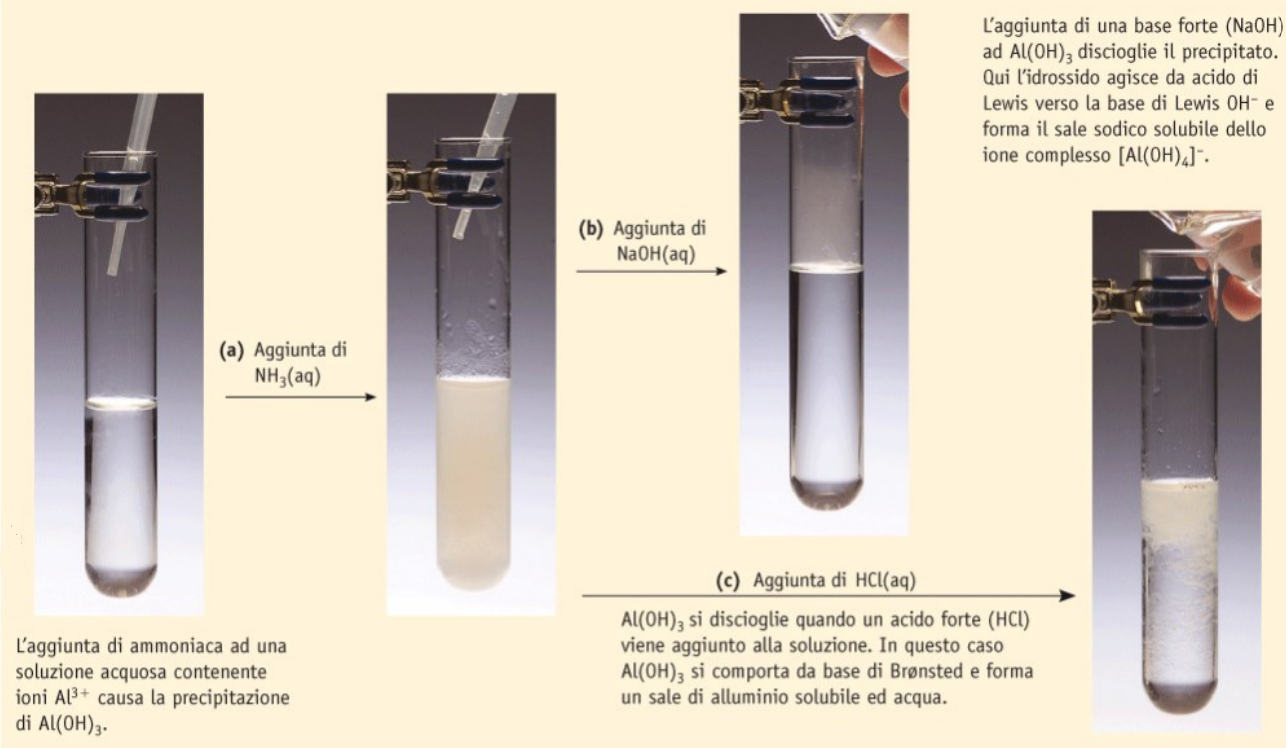
\includegraphics[width=12cm]{immagini/anfoliti.png}
\end{figure}

Immaginiamo di avere un sale di alluminio solubile in acqua. Se fosse in soluzione non ce ne accorgeremmo, in quanto la soluzione sarebbe limpida e incolore. Se aggiungiamo ammoniaca, che è una base, si forma un precipitato gelatinoso bianco, che è l'idrossido di alluminio.

L'$\rm Al(OH)_3$ si è formato dopo aver aggiunto l'ammoniaca che è una base debole, ossia non si dissocia totalmente.

Immaginiamo di aggiungere un'ulteriore base, questa però più forte. Essa sarà l'idrossido di sodio NaOH. Ci si accorge che il precipitato ottenuto prima si risolubilizza, si riscioglie, e la soluzione sarà di nuovo limpida e incolore. Ciò succede perché

$$\ce{NH_3 + H_2O <--> NH_4^+ OH^-}$$

$$\ce{Al(OH)_3(aq) + NaOH <--> [Al(OH)_4]^- + Na^+}$$

$$\ce{Al(OH)_3(aq) + 3HCl -> AlCl_3 + 3H_2O}$$
\subsection{Reazioni acido-base}
Reazioni in cui mettiamo a reagire un acido e una base.

Esempi:

\vspace{0.2cm}\ce{HCl(aq) + NH_3(aq) <--> NH_4^+(aq) + Cl^-(aq)}

\begin{center}
    \begin{tabular}{llllllll}
        \textbf{Nome} & \textbf{Acido 1} & & \textbf{Base 2} & & \textbf{Base 1} & & \textbf{Acido 2}\\[0.3ex]
        Acido cloridico & HCl & + & $\rm H_2O$ & \ce{<-->} & $\rm Cl^-$ & + & $\rm H_3O^+$\\[0.3ex]
        Acido nitrico & $\rm HNO_3$ & + & $\rm H_2O$ & \ce{<-->} & $\rm NO_3^-$ & + & $\rm H_3O^+$\\[0.3ex]
        Acido carbonico & $\rm H_2CO_3$ & + & $\rm H_2O$ & \ce{<-->} & $\rm HCO_3^-$ & + & $\rm H_3O^+$\\[0.3ex]
        Acido acetico & $\rm CH_3CO_2H$ & + & $\rm H_2O$ & \ce{<-->} & $\rm CH_3CO_2^-$ & + & $\rm H_3O^+$\\[0.3ex]
        Acido cianidrico & $\rm HCN$ & + & $\rm H_2O$ & \ce{<-->} & $\rm CN^-$ & + & $\rm H_3O^+$\\[0.3ex]
        Acido solfidrico & $\rm H_2S$ & + & $\rm H_2O$ & \ce{<-->} & $\rm HS^-$ & + & $\rm H_3O^+$\\[0.3ex]
        Ammoniaca & $\rm H_2O$ & + & $\rm NH_3$ & \ce{<-->} & $\rm OH^-$ & + & $\rm NH_4^+$\\[0.3ex]
        Ione carbonato & $\rm H_2O$ & + & $\rm CO_3^{2-}$ & \ce{<-->} & $\rm OH^-$ & + & $\rm HCO_3^-$\\[0.3ex]
        Acqua & $\rm H_2O$ & + & $\rm H_2O$ & \ce{<-->} & $\rm OH^-$ & + & $\rm H_3O^+$\\[0.3ex]
    \end{tabular}
\end{center}
\subsection{Forza degli acidi e delle basi}
\textbf{ES.}

$$\ce{HCOOH(aq) + H_2O(l) <--> HCOO^-(aq) + H_3O^+(aq)}$$

L'acido formico in acqua dà lo ione formiato, e il protone che si libera si associa all'acqua per formare $\rm H_3O^+$.
\subsection{Autodissociazione dell'acqua}
Abbiamo visto la reazione

$$\ce{H_2O + H_2O <--> H_3O^+ + OH^-}$$

In essa stiamo immaginando di avere soltanto acqua a disposizione. Ciononostante l'acqua si autodissocia producendo, tramite un equilibrio, un po' di ioni $\rm H_3O^+$ e un po' di ioni $\rm OH^-$.

Se così fosse l'acqua pura dovrebbe condurre. Con una misura di conducibilità possiamo risalire alla concentrazione di questi ioni. Vedremo che essa è molto piccola, per cui l'autodissociazione dell'acqua sarà trascurabile.

La costante è data da

$$\ce{2 H_2O <--> H_3O^+ + OH^-}
\implies
k= \frac{[\text{H}_3\text{O}^+] [\text{OH}^-]}{[\text{H}_2\text{O}]^2} \; (=1.8 \cdot 10^{-16})$$

$$\implies k \cdot [\text{H}_2\text{O}]^2 = [\text{H}_3\text{O}^+] \cdot [\text{OH}^-] = k_w$$

Poniamo $k_w$ il prodotto di $k$ per la concentrazione dell'acqua all'equilibrio al quadrato, che si vede essere pari anche al prodotto della concentrazione dello ione $\rm H_3O^+$ per quella dello ione $\rm OH^-$. Inoltre quest'ultime due concentrazioni saranno uguali, perché ogni due molecole di acqua si producono uno ione $\rm H_3O^+$ e uno ione $\rm OH^-$. Si trova infatti che entrambe sono pari a $10^{-7}$ mol/L.

Va da notare che se le quantità degli ioni sono uguali, non ci sarà un eccesso di $\rm H_3O^+$ che porta l'acqua ad essere acida né un eccesso di ioni $\rm OH^-$ che porta l'acqua ad essere basica: l'acqua è neutra, poiché questi ioni hanno stessa concentrazione.

\subsection{Titolazione acido forte-base forte}